\chapter{序}

按理来说,对于所谓「Z 世代」的年轻人,熟练地使用电脑应该是他们的生活必备技能。

但事实却并非如此。据我们观察,许多同学对电脑的使用也并不熟悉,甚至可以说是陌生:

\begin{itemize}
  \item 让他们去下载软件,有的同学可能会下载到各种「\textbf{P2P 高速下载器}」,弄得满机器流氓软件\CJKsout{(堪称下崽器);}
  \item 给他们一个 \texttt{zip} 或 \texttt{7z} 文件,一些同学可能压根不知道什么是「\textbf{压缩文件}」,什么是「\textbf{解压缩}」;
  \item 一些同学电脑上\textbf{装了四五个浏览器、三四个杀毒软件},「QQ 浏览器」「360 浏览器」相互掐架、「360 安全卫士」「2345 电脑管家」互相攻击\CJKsout{(养蛊);}
  \item 问他们自己电脑是什么\textbf{系统}、什么 \textbf{CPU},他们中一些甚至答不出「Windows」「macOS」,更别说「酷睿」「锐龙」这样的词语了;
  \item 甚至有一些同学会对着下图感慨「电脑\textbf{内存}又不够了」……
\end{itemize}

\begin{figure}[htb!]
  \centering
  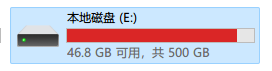
\includegraphics[width=6cm]{assets/Storage_Shortage.png}
\end{figure}

这或许是由于智能手机的普及造成的。
显然,使用电脑与使用手机相比,「复杂」了不止一个数量级。
然而,尽管几年前就有人说「电脑现在已经是夕阳产业了」,但事实却是:
至少在当下,我们仍然得学会去用电脑,不说多么「精通」,但至少要能知道\textit{软件怎么装、出现小问题怎么办、XX 文件怎么打开、怎么把文件打包}等等这些「21 世纪的常识」。

中小学的《信息技术》课堂、大学的《大学计算机基础》课程本应起到教授这些知识的作用。
可惜,事与愿违——很多时候,我们在这些课堂上学到的东西,可能一辈子都用不到;
真正需要学的东西,却缺失了:

我们一辈子可能也不会再尝试用 Excel 排出张三李四不及格的科目有哪些,不会再折腾复杂到毫无意义的页眉和页脚,不会再碰和动画制作和网页相关的任何内容。
但我们未来必然有无数次会需要去网上下载一个新的软件,会无数次遇到各种各样的软件错误、闪退或者崩溃,会无数次因为 Windows 更新导致这样或那样的问题,会无数次遇到电脑沾上垃圾软件而奇慢无比无法使用……

这份《Your Missing Semester of Using Computer》是一份为「电脑小白」准备的电脑操作指南。
它直译过来就是《你缺失的那门计算机课》,也可以叫做《你本应学过的计算机课》。
我们会假定读者基本不了解电脑的操作,换言之就是所谓「电脑小白」,告诉读者「电脑最好怎么用」。

这份教程会在文中简称自己为《Missing》。
《Missing》的得名参考了 MIT 的《\href{https://missing.csail.mit.edu/}{The Missing Semester of Your CS Education}》。